\section{Regulador experto}
\label{sec:reg_expt}

Durante las producciones realizadas anteriormente, se ha notado que existe una relación entre la velocidad de tracción y el diámetro final del filamento, sin embargo, el sistema que se dispone carece de la robustez necesaria para poder trabajar con un regulador del tipo PID, en el que es necesario conocer de manera lo más exacta posible, la distribución de la planta con la que se trabaja.\\

Como se ha visto en los ensayos anteriores, la salida de filamento que proporciona el filastruder no es constante y en ocasiones, no está bien mezclada.

\begin{figure}[H]
    \centering
    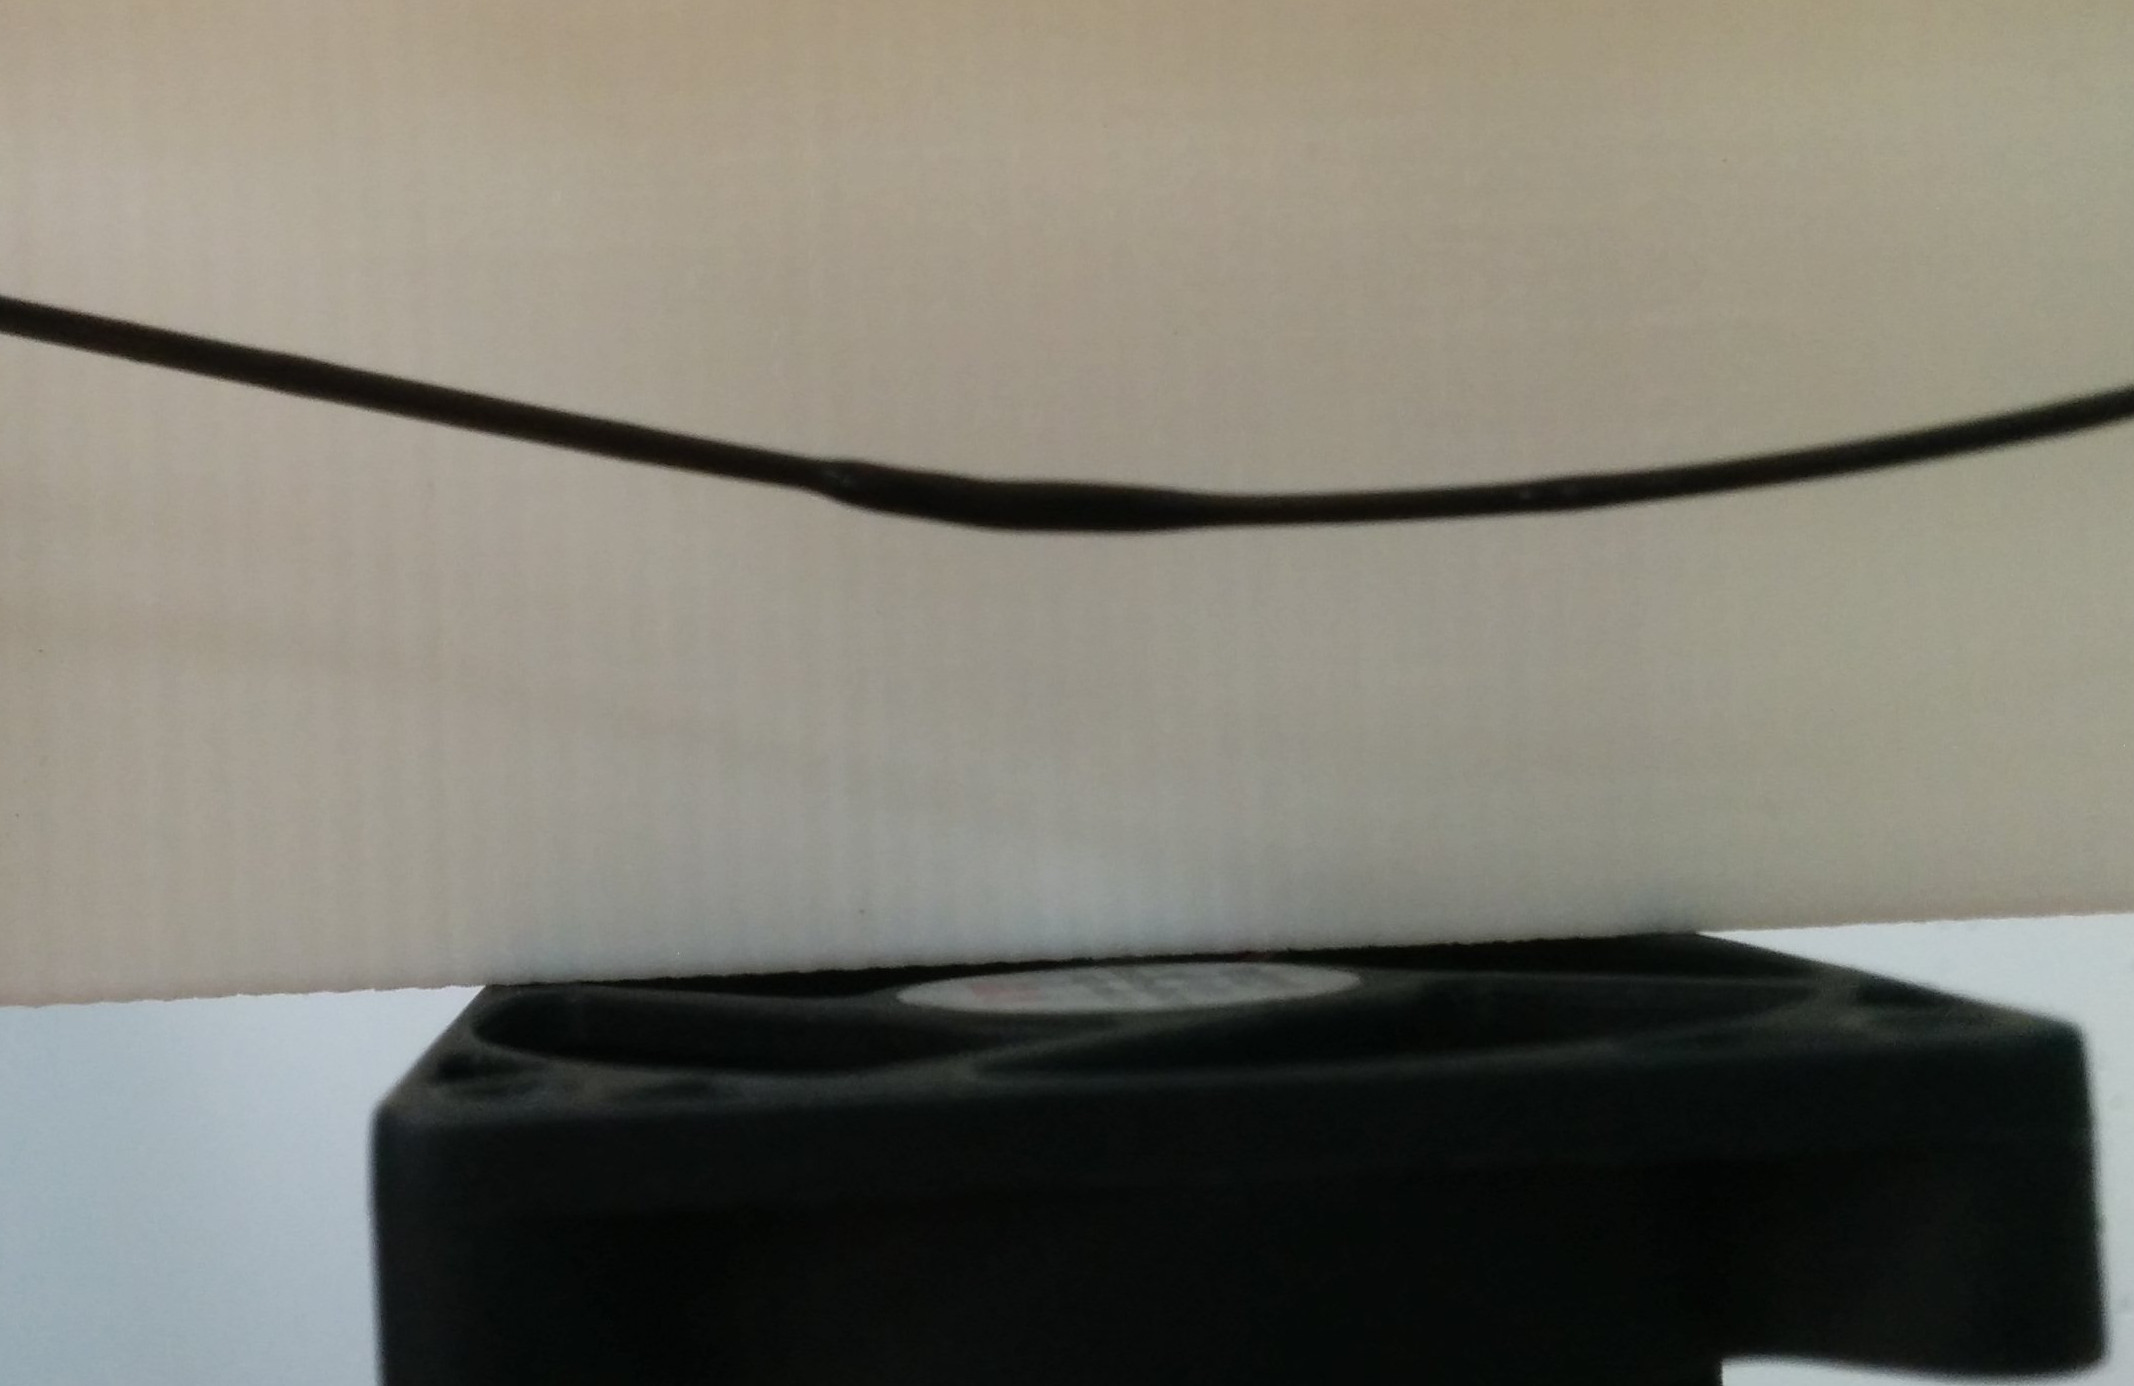
\includegraphics[width=0.6\textwidth]{images/producciones/22072015/IMG_20150722_120959.jpg}
    \caption{Mezcla incorrecta de la filastruder}
    \label{fig:reg_mezcla}
\end{figure}

Por ello, se decide no usar un regulador PID e intentar implementar un regulador experto, el cual, imitará las acciones que un humano tomaría para resolver el problema. Este tipo de reguladores se basan en un conocimiento previamente adquirido por una persona, que ha trabajado con el sistema.\\

Para implementear este sistema, se definen una serie de reglas, en las que acotaremos los diámetros del filamento en regiones, y dependiendo, de si el diámetro crece o decrece, se actuará sobre la velocidad de tracción
\begin{figure}[H]
    \centering
    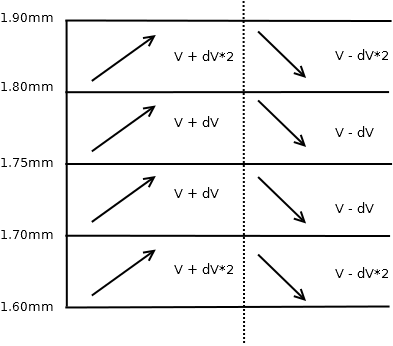
\includegraphics[width=0.5\textwidth]{images/producciones/11082015/Diagram1.png}
    \caption{Reglas a utilizar en el sistema experto}
    \label{fig:reg_reglas}
\end{figure}

Se realiza un bloque de programación que implemente esta filosifía y en función del diáemtro actual, y el diámetro anterior, se irá modificando la velocidad de tracción, para así variar el diámetro del filamento.\\

Una vez realiado el programa, se van a realizar varios ensayos con distintos parámetros para ver cómo influye el regulador.

\subsection{Ensayo 1}

Los datos con los que se realizaron el experimento fueron:

\begin{itemize}
	\item{Hora de inicio: 14:27}
	\item{Hora final : 15:08}
	\item{Filamento extruido: 537cm}
	\item{Granza de PLA mezcla: 70\% granza, 30\% pellets.}
	\item{Mezcla secada en horno 4 horas antes del ensayo.}
	\item{$T: 150ºC$}
	\item{$V_{min} tractora: 1.5 mm/s$}
	\item{$V_{max} tractora: 3.4 mm/s$}
	\item{Los incrementos de velocidades en las reglas del sistema experto son las mismas.}
\end{itemize}

Los resultados obtenidos son los siguientes:

\begin{table}[H]
	\centering
	\begin{tabular}{cc}
		                    & Diámetro X \\ \hline
		Medidas             & 1526       \\
		Media (mm)          & 1.72       \\
		Desviación estandar & 0.29       \\
		Mínimo (mm)         & 1.20       \\
		Máximo (mm)         & 2.56      
	\end{tabular}
	\caption{Datos obtenidos en el ensayo 1}
	\label{tab:resl_ens1}
\end{table}

Cómo vemos en la tabla \ref{tab:resl_ens1} la media del filamento conseguido es de $1.72 mm$, sin embargo, los valores límites de $1.65 mm$ y $1.85 mm$ han sido superados, por lo que el filamento que se ha extruido, no valdría en su totalidad para imprimir. Si representamos los datos obtenidos en una gráfica, podemos observar como hay una influencia del regulador. Las variaciones que hay en el diámetro, son no son tan pronunciadas como en el caso del funcionamiento en lazo abierto. \\

Con el gráfico de cajas, podemos ver que la distribución de los datos no es del todo homogena, teniendo una gran cantidad de los datos por encima de la media, sobre $1.96 mm$.

\begin{figure}[H]
    \centering
    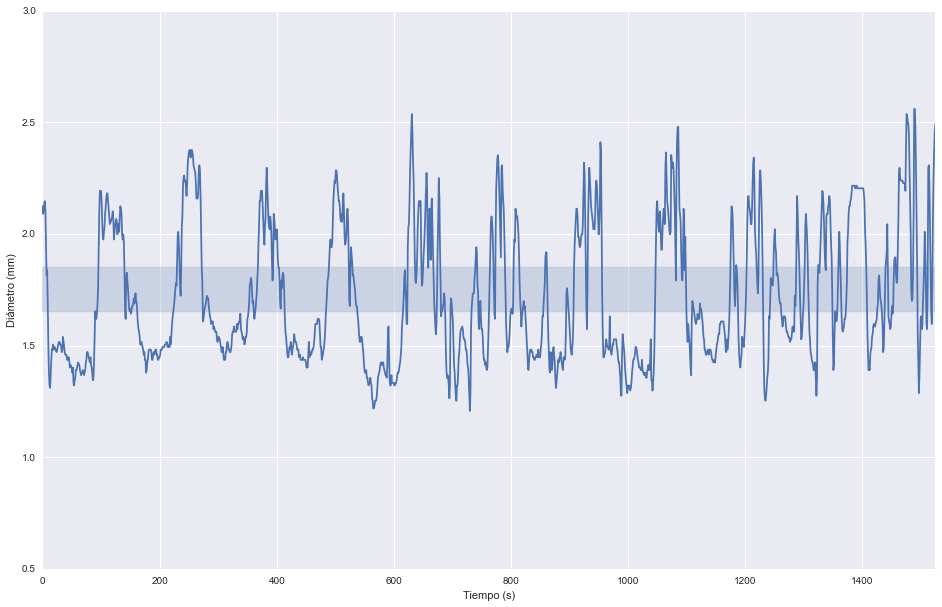
\includegraphics[width=0.99\textwidth]{images/producciones/11082015/output_9_1.png}
    \caption{Datos graficados del ensayo 1 con regulador experto}
    \label{fig:reg_graf}
\end{figure}

\begin{figure}[H]
    \centering
    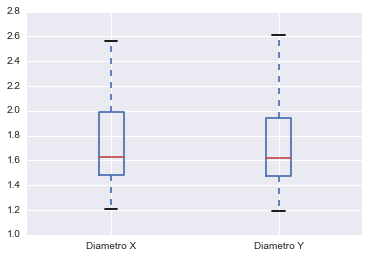
\includegraphics[width=0.6\textwidth]{images/producciones/11082015/output_10_1.png}
    \caption{Diagrama de cajas del ensayo 1 con regulador experto}
    \label{fig:reg_cajas}
\end{figure}

Como segunda aproximación que vamos a realizar será la de hacer mayores incrementos al subir la velocidad en los tramos que el diámetro se encuentre entre $1.80 mm$ y $1.75 mm$ haremos incrementos de velocidad mayor.

\subsection{Ensayo 2}

Los datos con los que se realizaron el experimento fueron:

\begin{itemize}
	\item{Hora de inicio: 11:05}
	\item{Hora final : 11:35}
	\item{Filamento extruido: 435cm}
	\item{$T: 150ºC$}
	\item{$V_{min} tractora: 1.5 mm/s$}
	\item{$V_{max} tractora: 3.4 mm/s$}
	\item{Los incrementos de velocidades en las reglas del sistema experto son distintas:}
\end{itemize}

En este ensayo, se va a cambiar el incremento de velocidad, cuando el filamento esté entre una diámetro de $1.75 mm$ y $1.80 mm$ y tenga una tendencia de crecimiento. Se hará que en este caso, la velocidad se incremente más.\\

Los resultados obtenidos son los siguientes:

\begin{table}[H]
	\centering
	\begin{tabular}{cc}
		                    & Diámetro X \\ \hline
		Medidas             & 1114      \\
		Media (mm)          & 1.74       \\
		Desviación estandar & 0.26       \\
		Mínimo (mm)         & 1.02       \\
		Máximo (mm)         & 2.45      
	\end{tabular}
	\caption{Datos obtenidos en el ensayo 2}
	\label{tab:resl_ens1}
\end{table}

Con los cambios realizados, los datos ahora son algo más estables, y hemos conseguido aumentar la media del filamento a $1.74 mm$ estando dentro del margen de producción, sin embargo, los límites superior e inferior no son los adecuados, alejándose demasiado de lo deseado. Sin embargo en este caso, una gran parte del filamento podría llegar a ser re-aprovechado para imprimir.

\begin{figure}[H]
    \centering
    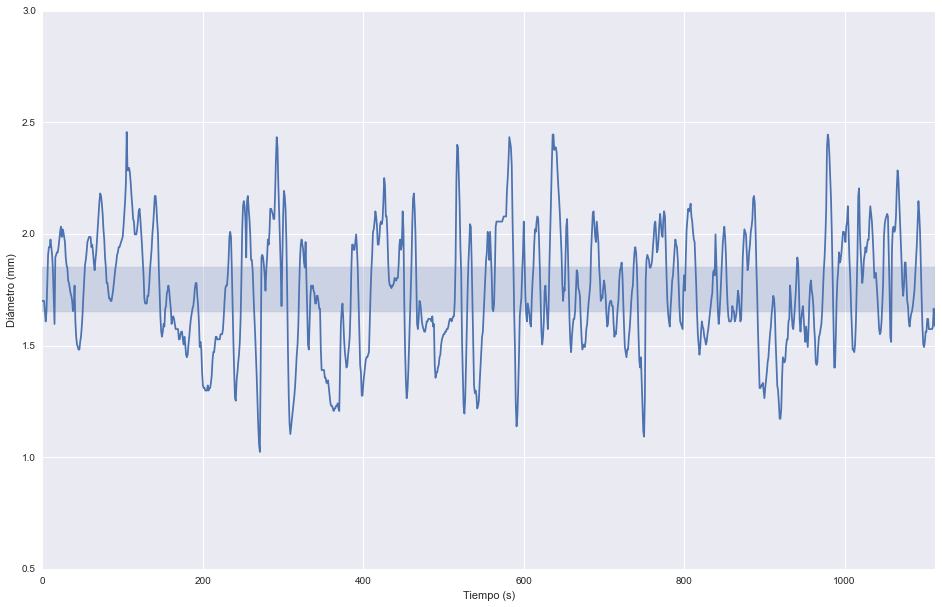
\includegraphics[width=0.99\textwidth]{images/producciones/12082015/output_9_e1.png}
    \caption{Datos graficados del ensayo 2 con regulador experto}
    \label{fig:reg_graf2}
\end{figure}

\begin{figure}[H]
    \centering
    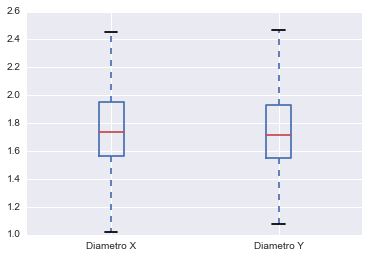
\includegraphics[width=0.6\textwidth]{images/producciones/12082015/output_10_e1.png}
    \caption{Diagrama de cajas del ensayo 2 con regulador experto}
    \label{fig:reg_cajas2}
\end{figure}

Como tercera aproximación, vamos a modificar los incrementos de velocidades en los tramos en los que el filamento se encuentre entre  $1.70 mm$ y $1.80 mm$

\subsection{Ensayo 3}

Los datos con los que se realizaron el experimento fueron:

\begin{itemize}
	\item{Hora de inicio: 12:00}
	\item{Hora final : 12:30}
	\item{Filamento extruido: 425cm}
	\item{$T: 150ºC$}
	\item{$V_{min} tractora: 1.5 mm/s$}
	\item{$V_{max} tractora: 3.4 mm/s$}
	\item{Los incrementos de velocidades en las reglas del sistema experto son distintas:}
\end{itemize}

En este ensayo, se va a cambiar el incremento de velocidad, cuando el filamento esté entre una diámetro de $1.75 mm$ y $1.80 mm$ y sea cual sea la tendencia. Se hará que en este caso, la velocidad se incremente más.\\

Los resultados obtenidos son los siguientes:

\begin{table}[H]
	\centering
	\begin{tabular}{cc}
		                    & Diámetro X \\ \hline
		Medidas             & 1124      \\
		Media (mm)          & 1.66       \\
		Desviación estandar & 0.24       \\
		Mínimo (mm)         & 0.98       \\
		Máximo (mm)         & 2.60      
	\end{tabular}
	\caption{Datos obtenidos en el ensayo 2}
	\label{tab:resl_ens1}
\end{table}

Con esta tercera aproximación se ha conseguido estabilizar los datos y reducir la desviación estandar, sin embargo, la media del filamento y de la velocidad de tracción ha disminuido también. Por lo tanto, los cambios realizados no han sido satisfactorio


\begin{figure}[H]
    \centering
    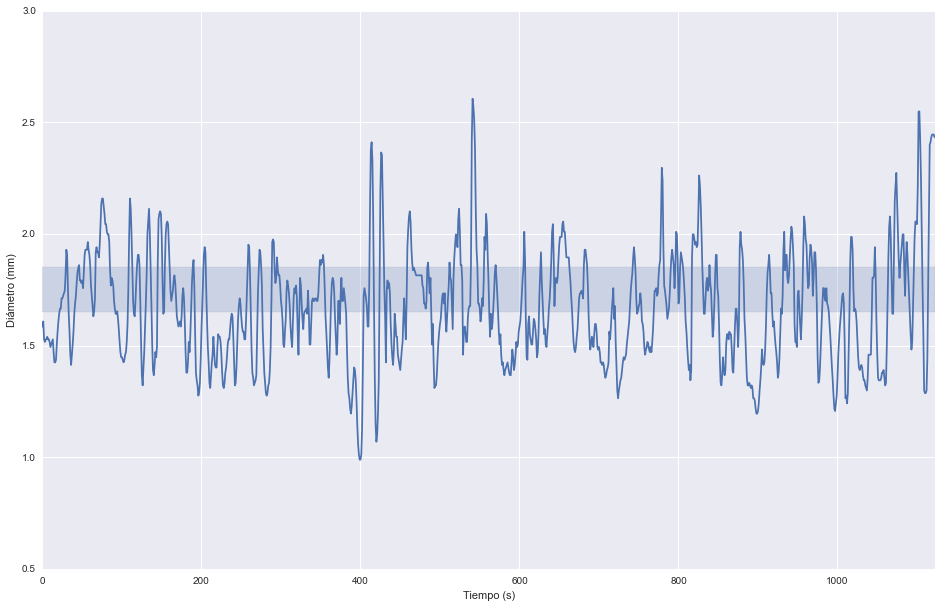
\includegraphics[width=0.99\textwidth]{images/producciones/12082015/output_9_e2.png}
    \caption{Datos graficados del ensayo 3 con regulador experto}
    \label{fig:reg_graf3}
\end{figure}

\begin{figure}[H]
    \centering
    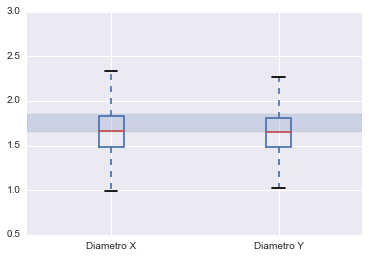
\includegraphics[width=0.6\textwidth]{images/producciones/12082015/output_10_e2.png}
    \caption{Diagrama de cajas del ensayo 3 con regulador experto}
    \label{fig:reg_cajas3}
\end{figure}

Como cuarta  aproximación, vamos a  modificar los incrementos en los que el diámetro se encuentra entre $1.70 mm$ y $1.80 mm$, en sentido de subida.En el sentido de bajada se mantendrá con incrementos de +1.\\

Se ha detectado también que el eje de giro de la tractora está algo suelto. Se va a apretar para el siguiente ensayo.\\
